\section{Manuel d'utilisation}

Cette application débute avec une boîte de dialogue qui laisse le choix entre deux rôles : Maître de Jeu (MJ) ou Joueur. Si "MJ" est choisi, l'application se lance en tant que serveur pour accueillir les joueurs. Si "Joueur" est choisi, un assistant ce connexion apparaît pour choisir à quel serveur se connecter. Dans les deux cas, un pseudonyme est demandé; si le champs n'est pas rempli la personne se nommera "guest".

\subsection{Chat}
L'interface qui se présente comporte un Chat, un gestionnaire de tours et le lanceur de dés. Le Chat contient la liste des utilisateurs et permet aux joueurs et au MJ de communiquer. De plus, le chat possède des commandes qui s'introduisent par un /. Les commandes implémentées sont :

\begin{description}
	\item[/help] \hfill \\
		Affiche l'ensemble des autres commandes disponibles du chat avec les indications d'utilisation.
	\item[/nickname <pseudo>] \hfill \\
		Modifie le pseudo par celui qui suit la commande.
	\item[/roll <nombre de dés>d<valeur max du dé>] \hfill \\
		Roule un nombre de fois voulu du dé choisi. Peut s'utiliser en chuchotement. Peut lancer de multiples dés en les séparant par un '+' ou un '-'. Peut ajouter une valeur fixe au résultat final en ne précisant pas la partie "d<valeur max du dé>.
	\item[/whisper <utilisateur> <message>] \hfill \\
		Envoie un message privé au joueur indiqué. Peut cibler des utilisateurs multiples en les séparant par '|'.
\end{description}

\begin{figure}[h!]
	\centering
	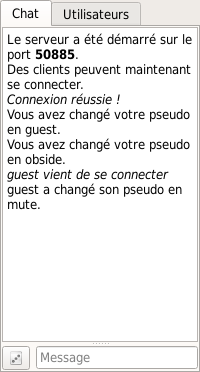
\includegraphics[scale=0.5]{img/chat_mj.png}
	\hspace{10 mm}
	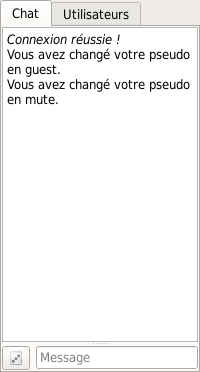
\includegraphics[scale=0.5]{img/chat_player.png}
	\caption{Chat MJ (à gauche) et chat Joueur (à droite)}
\end{figure}

Le Chat propose également une liste d'utilisateurs connectés. Un clic droit sur un ou plusieurs utilisateurs de cette liste affiche un menu contextuel donnant accès à des actions : Envoyer un message, et Lancer les dés.
La première action prépare un message privé à un ou plusieurs utilisateurs, la seconde lance les dés sélectionnés dans le lanceur de dés et envoie le résultat uniquement aux utilisateurs sélectionnés.


\begin{figure}[h!]
	\centering
	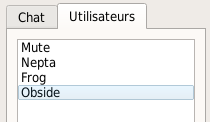
\includegraphics[scale=0.5]{img/chat_userlist_1.png}
	\hspace{10 mm}
	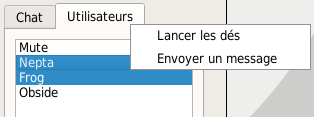
\includegraphics[scale=0.5]{img/chat_userlist_2.png}
	\caption{Liste d'utilisateurs (à gauche) et menu contextuel proposant des actions sur les utilisateurs sélectionnés (à droite)}
\end{figure}
\newpage

\subsection{Lanceur de dés}
Le lanceur de dés propose les dés les plus utilisés et permet de choisir pour chaque type de dé, le nombre de fois que celui-ci doit être lancé. Initialement, les compteurs sont à zéro. Pour augmenter le nombre dés à lancer, il faut effectuer un clic gauche sur le bouton correspondant ou utiliser la molette de la souris pour faire varier le nombre en étant sur le bouton. De même, pour décrémenter les dés il suffit de cliquer droit ou de faire défiler la molette vers le bas sur un bouton. On peut ensuite décider de lancer les dés sur le chat (lancé public) ou de lancer les dés en privé (lancé caché). Un lancé privé n'est visible que par celui qui l'effectue, et est principalement utilisé par le MJ. Il est également possible de réinitialiser tous les compteurs.

\begin{figure}[h!]
	\centering
	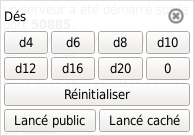
\includegraphics[scale=0.5]{img/dice_manager.png}
	\caption{Lanceur de dés}
\end{figure}

\subsection{Gestionnaire de tours}
Le gestionnaire de tours est un outil qui permet au MJ de gérer ses combats. Les icônes sur la droite du gestionnaire permettent d'ajouter et de retirer des tours à la liste (voir figure \ref{fig:turnManager}). Ceux-ci peuvent par exemple représenter les tours des personnages joueurs, non joueurs et/ou des lancers de sorts. Le MJ peut également réordonner les tours à l'aide du glisser-déposer. Toutes les actions effectuables à la souris disposent également d'un équivalent en raccourcis clavier, il est par exemple possible de naviguer entre les tours et de les réarranger à l'aide des flèches du clavier. Pour sélectionner plusieurs éléments à l'aide du clavier, il suffit de maintenir la touche Maj enfoncée et d'appuyer sur les flèches. Pour en déplacer, il suffit d'en sélectionner puis de mainternir la touche Ctrl enfoncée et d'appuyer sur les flèches. Enfin, lorsque des utilisateurs se connectent ils sont automatiquement ajoutés dans le gestionnaire de tour.

\begin{figure}[h!]
	\centering
	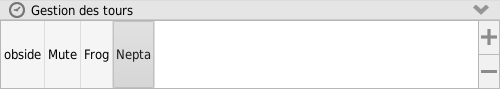
\includegraphics[width=0.7\textwidth]{img/turn_manager.png}
	\caption{Gestionnaire de tour}
	\label{fig:turnManager}
\end{figure}
\newpage

\subsection{Liste de jetons}
La liste des jetons (figure \ref{fig:tokenmenu}) répertorie les jetons qui peuvent être posés sur une carte. Il est possible d'ajouter des jetons personnalisés, c'est à dire des jetons avec un texte indiqué dessus. Des jetons possédant un élément de jeu peuvent également être ajoutés via une fenêtre d'édition d'élément de jeu (figure \ref{fig:gameobject_edit}). Les seuls éléments de jeu disponibles à l'heure actuelle sont les personnages (qui sont caractérisés par des points de vie).

\begin{figure}[h!]
	\centering
	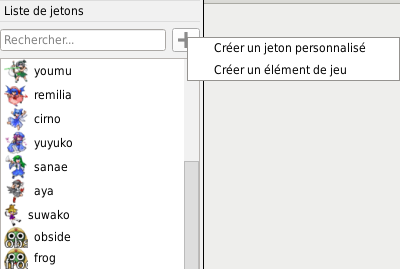
\includegraphics[width=0.5\textwidth]{img/tokenmenu.png}
	\caption{Liste de jetons et options d'ajout de jetons}
	\label{fig:tokenmenu}
\end{figure}

\begin{figure}[h!]
	\centering
	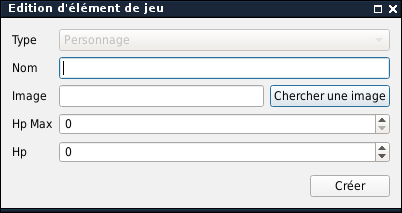
\includegraphics[width=0.5\textwidth]{img/gameobject_edit.png}
	\caption{Fenêtre d'édition d'un élément de jeu}
	\label{fig:gameobject_edit}
\end{figure}
\newpage

\subsection{Carte et images}

La carte et les images sont les deux éléments centraux de notre application. Elles servent à émuler respectivement le plateau de jeu (souvent une planche velleda quadrillée sur laquelle on place des figurines) et de simples feuilles papier sur lesquelles les participants peuvent dessiner.\\
Leurs utilisations réelles étant relativement proches l'une de l'autre, nous avons fait le choix de leur attribuer des comportements similaires. L'utilisateur peut dessiner sur une carte ou une image, mais ne peut ajouter des jetons ou du brouillard de guerre que sur une carte.

\subsubsection{Création et ouverture d'une carte ou d'une image}

Dans le menu principal, section "Partie", choisir "Créer une carte" ou "Créer une image". Une fenêtre apparaît alors, demandant de choisir un fichier d'image qui servira d'arrière-plan. \\
Il faut ensuite nommer la carte (ce nom servira à nommer la fenêtre de la carte et à sauvegarder la carte) et choisir une tailler pour le quadrillage. Si l'utilisateur choisit une taille de 1, alors les cases ne seront pas dessinées.\\

Toutes les modifications que l'utilisateur peut effectuer sur une carte ou une image sont directement sauvegardées dans la base de données. Ainsi, après la fermeture d'une fenêtre ou de l'application, l'utilisateur peut retrouver sa carte dans le même état (jetons et dessins compris) en allant dans le menu "Partie"/"Ouvrir une carte/image".

\subsubsection{Présentation rapide de la fenêtre}

Une vue centrale affiche l'image ou la carte, et un menu sur la droite  permet de choisir ce que l'on souhaite afficher ou modifier, et donne accès aux outils associés à la sélection. Ce menu peut se rabattre afin de libérer plus d'espace visible sur la carte.\\
Le menu de droite contient trois section principales:
\begin{description}
	\item[Affichage]: permet de sélectionner les couches que l'on souhaite afficher. Seul le maître du jeu peut choisir de cacher le brouillard de guerre.
	\item[Sélecteur de couche]: permet de sélectionner la couche dans laquelle on souhaite travailler. Seul le maître du jeu peut modifier le brouillard de guerre, afin d'éviter les abus de la part des joueurs.
	\item[Outils]: changent selon la couche que l'on édite. Permet d'accéder aux outils agissant sur ladite couche.
\end{description}


\begin{figure}[h!]
	\centering
	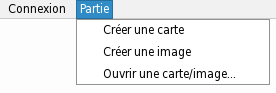
\includegraphics[scale=0.9]{img/create_map_menu.png}
	\caption{Menu de création et d'ouverture}
    \label{fig:createmapmenu}
\end{figure}



\subsubsection{Gestion des jetons}

Afin d'accéder à la gestion des jetons, il faut cocher la case "Carte" dans le sélecteur de couche. Lorsque cette couche est sélectionnée, l'utilisateur peut: 
\begin{description}
	\item[Changer l'échelle]: dans le menu outil, utiliser le slider pour zoomer ou dézoomer.
	\item[Ajouter un jeton]: au relâchement du clic gauche sur un emplacement quelconque de la carte, le jeton sélectionné dans la liste de jetons sera ajouté à la carte et aligné avec la grille. Il est aussi possible de drag and drop un jeton depuis la liste de jetons. Il est aussi possible d'ajouter des jetons en continu sur les cases n'en possédant pas encore en cliquant sur une case libre puis en déplaçant le curseur.
	\item[Supprimer un jeton]: lors du clic droit sur un jeton, un menu apparaît proposant de supprimer ledit jeton. Il est aussi possible de les supprimer en continu de la même manière que pour l'ajout en continu, mais en cliquant droit.
	\item[Déplacer un jeton]: il est possible de drag and drop les jetons avec un clic gauche. Lors du déplacement, la distance la plus courte à parcourir est affichée dans le coin inférieur droit. Cette distance est calculée selon les règles officielles de Pathfinder.
	\item[Modifier les points de vie d'un jeton]: faire un clic droit sur un jeton, choisir "Editer le personnage", et modifier les points de vie. Il est possible de choisir un montant de points de vie négatif.
	\item[Consulter les informations sur une case]: lorsque l'on passe sur une case, une info-bulle s'affiche dans le coin inférieur droit indiquant le nombre de jetons présents sur la case. De plus, si le jeton supérieur a des points de vie, alors ils sont affichés sous la forme d'un cercle autour de la case (voir figure \ref{fig:lifebar}). Les points de vie sont rouges s'ils sont positifs et bleus s'ils sont négatifs.
\end{description}

\begin{figure}[h!]
	\centering
	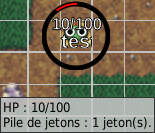
\includegraphics[scale=0.9]{img/gameobject_lifebar.png}
	\caption{Barre de vie d'un sprite posé sur la carte}
    \label{fig:lifebar}
\end{figure}


\subsubsection{Gestion du brouillard de guerre}

Lors d'une séance de jeu de rôle, il est indispensable que le maître du jeu puisse dissimuler des informations aux joueurs. Nous avons donc choisi d'utiliser le concept de brouillard de guerre, très répandu dans les jeux de stratégie: les cases que les joueurs ne peuvent pas voir sont recouvertes de gris opaque. Seul le MJ peut ajouter, retirer ou ne pas afficher le brouillard de guerre. Le brouillard de guerre est transparent pour le MJ. Il lui est possible de complètement remplir ou retirer le brouillard de guerre depuis les boutons de la section Outil.


\begin{figure}[h!]
	\centering
	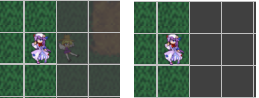
\includegraphics[scale=0.9]{img/FoW_Compare.png}
	\caption{A gauche, vision du MJ; à droite, vision d'un joueur}
    \label{fig:fowcompare}
\end{figure}

\subsubsection{Gestion des dessins}

Lors d'une partie de jeu de rôle papier, il est possible de dessiner sur les cartes pour ajouter des éléments imprévus (un mur effondré, un piège,...). De plus, il est possible pour les joueurs de désigner des éléments, ce qui est compliqué à distance. C'est pour cela que nous avons créé cette couche.

\begin{description}
	\item[Dessiner]: Cette option est sélectionnée par défaut. Il faut cliquer sur le bouton "Crayon", puis cliquer gauche sur la carte. tant que le bouton gauche de la souris est maintenu, on continue à dessiner. Il est possible de dessiner des lignes en maintenant la touche Shift. Une ligne peut alors être prévisualisée, et est dessinée lors du relâchement de la touche Shift ou de la souris.
	\item[Effacer]: Appuyer sur le bouton "Gomme", puis cliquer droit sur la carte. Pour effacer tous les dessins, appuyer sur le bouton "Effacer dessins".
	\item[Modifier l'épaisseur des traits]: respectivement pour la gomme et la souris, utiliser les champs "Crayon" et "Gomme".
	\item[Partager les dessins]: les dessins ne sont partagés avec les autres joueurs qu'une fois le bouton "Envoyer" cliqué.
	\item[Envoyer un signal]: choisir l'outil "ping", puis cliquer sur la carte. Une animation est alors jouée à cet emplacement pour tous les joueurs. Il n'est pas nécessaire d'envoyer les dessins pour partager le ping. Cet élément s'inspire des jeux de stratégie en équipe, et sert aux utilisateurs à désigner les objectifs.
\end{description}

\subsubsection{Les logs}

Afin que le MJ puisse connaître les actions effectuées par les joueurs sans avoir à regarder tout le temps son écran, nous avons implementé une  liste de logs.

Grâce à cela, le MJ peut surveiller les abus éventuels des joueurs, pour cela, dans le widget des différents token disponible, un onglet sous la forme d'un accordéon se nomme \og Historique\fg{}, il suffit de cliquer dessus pour faire apparaître les dernières actions effectuées.

\begin{figure}[h!]
    \centering
    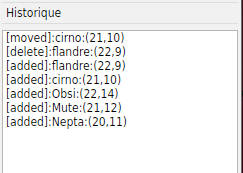
\includegraphics[scale=0.7]{img/log.png}
    \caption{historique}
    \label{fig:log}
\end{figure}


